\documentclass[11.5pt]{sig-alternate} % sets document style to sig-alternate
% packages
% typesetting
%\usepackage{dirtytalk} % typset quotations easier (\say{stuff})
\usepackage{hanging} % hanging paragraphs
\usepackage[defaultlines=3,all]{nowidow} % avoid widows
\usepackage[pdfpagelabels=false]{hyperref} % produce hypertext links, includes backref and nameref
\usepackage{xurl} % defines url linebreaks, loads url package
\usepackage{microtype}
\usepackage[super]{nth} % easily create superscript ordinal numbers with \nth{x}
% layout
\usepackage{enumitem} % control layout of itemize, enumerate, description
\usepackage{fancyhdr} % control page headers and footers
\usepackage{float} % improved interface for floating objects
%\usepackage{multicol} % intermix single and multiple column pages
% language
\usepackage[utf8]{inputenc} % accept different input encodings
\usepackage[english]{babel} % multilanguage support
% misc
\usepackage{graphicx} % builds upon graphics package, \includegraphics
%\usepackage{lastpage} % reference number of pages
%\usepackage{comment} % exclude portions of text (?)
\usepackage{xcolor} % color extensions
\usepackage[backend=biber, style=apa]{biblatex} % sophisticated bibliographies % necessary for HTML to display author info and date on abstract page
\usepackage{csquotes} % advanced quotations, makes biblatex happy
\usepackage{authblk} % support for footnote style author/affiliation
% tables and figures
\usepackage{tabularray}
%\usepackage{array} % extend array and tabular environments
\usepackage{caption} % customize captions in figures and tables (rotating captions, sideways captions, etc)
%\usepackage{cuted} % allow mixing of \onecolumn and \twocolumn on same page
\usepackage{multirow} % create tabular cells spanning multiple rows
%\usepackage{subfigure} % deprecated, support for manipulation of small figures
%\usepackage{tabularx} % extension of tabular with column designator "x", creates paragraph-like column whose width automatically expands
%\usepackage{wrapfig} % allows figures or tables to have text wrapped around them
%\usepackage{booktabs} % better rules
% dummy text
%\usepackage{blindtext} % blind text dummy text
%\usepackage{kantlipsum} % Kant style dummy text
\usepackage{lipsum} %lorem ipsum dummy text
% other helpful packages may be booktabs, longtable, longtabu, microtype

\pagestyle{fancy} % sets pagestyle to fancy for fancy headers and footers

% header and footer
% modern way to set header image
\renewcommand{\headrulewidth}{0pt} % defines thickness of line under header
\renewcommand{\footrulewidth}{0pt} % defines thickness of line above header
\setlength\headheight{80.0pt} % sets height between top margin and header image, effectively moves page contents down
\addtolength{\textheight}{-80.0pt} % seems to affect the lower height. maybe only works properly if footer numbers enabled?
\fancyhf{}
\fancyhead[CE, CO]{
\includegraphics[width=\textwidth]{headerImage.png}}
% footer
%\fancyfoot[LE,LO]{Article Title Here \\ DOI: }% left footer article title and doi
%\fancyfoot[CE,CO]{{}} % center footer empty
%\fancyfoot[RE,RO]{\thepage} % right footer page numbers
%\pagenumbering{arabic} % arabic (1, 2, 3) numbering in footer

\hypersetup{colorlinks=true,urlcolor=blue} % sets link color to blue
\urlstyle{same} % sets url typeface to same as rest of text

% set caption and figure to italics, label bold, left align captions, does not transfer to HTML
\DeclareCaptionFormat{custom}
{
    \textbf{\textit{\large #1#2}}\textit{\large #3} % #1 is the "Table 1" or "Figure 1" part, #2 is the separator (":"), #3 is the caption
}
\captionsetup{format=custom}
\captionsetup{justification = raggedright, singlelinecheck = false}

%this next bit is confusing, but essentially changes the width of the abstract. Seems to have been copied from this https://tex.stackexchange.com/questions/151583/how-to-adjust-the-width-of-abstract
\let\oldabstract\abstract
\let\oldendabstract\endabstract
\makeatletter %changes @ catcode to enable modification (in parsep)
\renewenvironment{abstract} %alters the abstract environment
{\renewenvironment{quotation}%
               {\list{}{\addtolength{\leftmargin}{1em} % change this value to add or remove length to the the default ?
                        \listparindent 1.5em%
                        \itemindent    \listparindent%
                        \rightmargin   \leftmargin%
                        \parsep        \z@ \@plus\p@}%
                \item\relax}%
               {\endlist}%
\oldabstract}
{\oldendabstract}
\makeatother %changes @ catcode to disable modification

\begin{document}

\title{TactViz: A VMD Plugin for Tactile Visualization of Protein Structures}

\author[1]{\large \color{blue}Olivia R. Shaw}
\author[1]{\large \color{blue}Jodi A. Hadden-Perill}
\affil[1]{Department of Chemistry and Biochemistry University of Delaware}

\toappear{}
%% ABSTRACT
\maketitle
\begin{@twocolumnfalse} 
\begin{abstract}
\item 
\textit {Scientific disciplines spanning biology, biochemistry, and biophysics involve the study of proteins and their functions. Visualization of protein structures represents a barrier to education and research in these disciplines for students who are blind or visually impaired. Here, we present a software plugin for readily producing variable-height tactile graphics of proteins using the free biomolecular visualization software Visual Molecular Dynamics (VMD) and protein structure data that is publicly available through the Protein Data Bank. Our method also supports interactive tactile visualization of proteins with VMD on electronic refreshable tactile display devices. Employing our method in an academic laboratory has enabled an undergraduate student who is blind to carry out research alongside her sighted peers. By making the study of protein structures accessible to students who are blind or visually impaired, we aim to promote diversity and inclusion in STEM education and research.} 
\\ \\
Keywords: Tactile Graphics, Tactile Visualization, Blind, Visually Impaired, Accessibility, Proteins, STEM
\end{abstract}
\end{@twocolumnfalse}

%% AUTHOR INFORMATION


\textbf{*Corresponding Author, Jodi A. Hadden-Perill }\\
\href{mailto: jhadden@udel.edu }{(jhadden@udel.edu)} \\
\textit{Submitted Mar 1 2020}\\
\textit{Accepted Apr 14 2020} \\
\textit{Published online Jul 24 2020} \\
\textit{DOI:10.14448/jsesd.12.0015} \\
\pagebreak
\clearpage

\begin{large}
 
\section*{INTRODUCTION}

\subsection*{Tactile Graphics}

Tactile graphics, 2-dimensional graphics that employ raised surfaces to convey non-textual information through touch, are a major physical medium used in the instruction of students who are blind or visually impaired (Edman, 1992). Also called relief representations, tactile graphics may be used to depict images, diagrams, schematics, flow charts, maps, or graphs. Along with verbal descriptions and tangible 3-dimensional models, tactile graphics provide a valuable complementary approach for communicating visual and topological details of a subject. Common methods for generating tactile graphics include embossing, vacuum or thermoforming, printing layered inks or substrates, and printing on specialized papers that expand when heated.

Tactile graphics methods based on the application of heat to swell or microcapsule paper are very popular due to convenience, low cost, and quick production (Rowell \& Ungar, 2003; Thompson \& Chronicle, 2006). Devices designed to produce these graphics include the Swell Form Machine, Picture In A Flash, and TactPlus. The application of heat to the specialized papers causes the regions of an image that are darkly shaded to swell, or elevate and become tactile (Hashimoto \& Watanabe, 2016). Darkly shaded regions elevate more than lightly shaded regions, such that elevation height (typically on the millimeter scale) can be tuned by controlling shading in a grayscale image. Along with textures, variable elevation height can be used to encode additional information into tactile graphics. Electronic refreshable tactile display devices, like the Graphiti, which use arrays of pins that raise and lower to show tactile graphics, may offer multiple pin heights to likewise enrich tactile visualization. 

Whatever the medium, conceptually clear tactile graphics can be challenging to create (Barth, 1982) and are less readily available for advanced subject material. Here, we present a strategy for generating images of proteins using free biomolecular visualization software and publicly available protein structure data that translate into comprehensible tactile graphics when printed with swell or microcapsule paper. An example ready-to-print tactile graphic featuring the protein GB1, produced using our method, is included in the Appendix.

\subsection*{Protein Structure and Visualization}

Proteins are essential biological molecules whose natural functions are governed by their 3-dimen\-sional shapes (Buxbaum, 2007). The shape of a protein is determined by its structure and the sensitivity of that structure to the surrounding environment (Chothia, 1984). Proteins are composed of linear chains of amino acids. Each protein has a unique amino acid sequence, called its primary structure. The primary structure folds locally to produce secondary structure elements, such as alpha-helices and beta-sheets. These elements further fold to give rise to the protein’s tertiary structure, and ultimately its 3-dimensional shape. The shape of a protein is a major factor underlying its physical properties and interactions with other biological molecules. Protein shape can vary with environmental conditions, such as temperature, pH,  or ionic strength, or upon binding of substrates, cofactors, or drug compounds.

Scientific disciplines spanning biology, biochemistry, and biophysics rely on knowledge of protein structure to elucidate the mechanisms by which proteins carry out their functions, as well as to identify strategies by which those functions can be improved or altered to treat disease and improve human health. Protein structure determination is a major field of research based on experimental techniques including X-ray crystallography, nuclear magnetic resonance (NMR) spectroscopy, and cryo-electron micros-copy (Dobson, 2019), and computational techniques including molecular modeling and molecular dynamics simulations (Goh et al., 2016). The many 3-dimensional protein structures that have been solved by researchers are systematically deposited in and freely available for download from the Research Collaboratory for Structural Bioinformatics (RCSB) Protein Data Bank (Berman et al., 2000): \url{https://www.rcsb.org/pdb/}

The investigation of protein structure and struc\-ture-function relationships often relies heavily on molecular visualization. Because the atomistic details of protein structures can be very difficult to inspect visually, numerous abstracted or simplified protein representations have been developed to improve visualization (Goebel, 2014). For example, the widely recognized Ribbon and Cartoon representations display only features of the protein backbone to illustrate, as clearly as possible, the global protein fold. Color schemes may further be applied to highlight secondary structure elements, such that alpha-helices, beta-sheets, and other local-fold aspects are distinct. Scientific software for advanced visualization of proteins and other biomolecular structures are readily available. For example, Visual Molecular Dynamics (VMD) (Humphrey et al., 1996) is a widely used, freely available software package for biomolecular visualization and analysis: \url{https://www.ks.uiuc.edu/Research/vmd/}

\subsection*{TactViz Brings Protein Structure to Tactile Graphics}

Visualization of protein structures represents a barrier to education and research for students who are blind or visually impaired. In remedy, we present a plugin for the VMD software to support tactile visualization of proteins. The plugin introduces representation schemes designed to produce variable-height tactile graphics, as well as drive interactive visualization on electronic refreshable tactile display devices. Through the development of this plugin, we aim to promote diversity and inclusion in STEM education and research by improving accessibility of protein structure visualization for individuals who are blind or visually impaired.

\section*{METHODS}

TactViz is a VMD plugin written in the TCL programming language. VMD runs on Windows, Mac, and Linux operating systems and is accessible to individuals who are blind or visually impaired through its text console interface, which can be used with a screen reader or Braille display. TactViz is freely available for download from GitHub: \url{https://github.com/jodihadden/TactViz/}

Loading TactViz into VMD applies a representation scheme and display settings that have been empirically optimized to produce clear tactile graphics of 3-dimensional protein structures. The New Cartoon representation provides an abstraction of the protein backbone that distinctly illustrates alpha-helices, beta-sheets, and loops in the protein secondary structure. TactViz takes advantage of VMD’s native shading capabilities to display the protein in grayscale, with the shading gradient indicating special depth. Regions of the structure that are closer to the viewer are more darkly shaded, and shading decreases with distance from the viewer. In keeping with the convention of tactile graphics, more darkly shaded regions will become more elevated and appear closer to the viewer. The sense of depth provided by variable tactile elevation height illuminates the 3-dimensional nature of the protein structure. Shading of the protein updates automatically upon rotation or reorientation, allowing inspection from any viewing angle.

To expand accessibility of VMD for individuals who are blind or visually impaired, as well as simplify usage for non-experts, TactViz also includes shortcuts for common actions, which can be executed through the text console. For example, commands for loading or deleting Protein Data Bank files, zooming in on or rotating the structure, toggling the projection mode between perspective and orthographic, rendering an image that can be printed as a tactile graphic, and rendering a stereolithography (STL) file that can be used for printing a 3-dimensional model are currently implemented. Commands are also implemented for adjusting the shading contrast and intensity in order to optimize the results produced by every individual’s available tactile graphics machine. TactViz is under active development and new features will continue to be added.

\section*{RESULTS AND DISCUSSION}

TactViz supports tactile visualization of proteins. Along with 3-dimensional printed models, variable-height tactile graphics produced using TactViz enable individuals who are blind or visually impaired to conceptualize and analyze protein structures through the sense of touch. Figure 1 shows four different approaches for visualization of the protein GB1, including a 3-dimensional printed model, a computer rendering produced using TactViz, a tactile graphic produced using TactViz, and tactile visualization on an electronic refreshable tactile graphics display, also powered by VMD with TactViz. The depth-based shading applied by TactViz translates to elevation height in tactile visualization to illuminate the 3-dimensional nature of the protein structure. A ready-to-print tactile graphic of the protein GB1 [PDB ID 2QMT (Schmidt et al., 2007)], produced using TactViz, is presented in the Appendix. 

\begin{figure}[h]
    \centering
    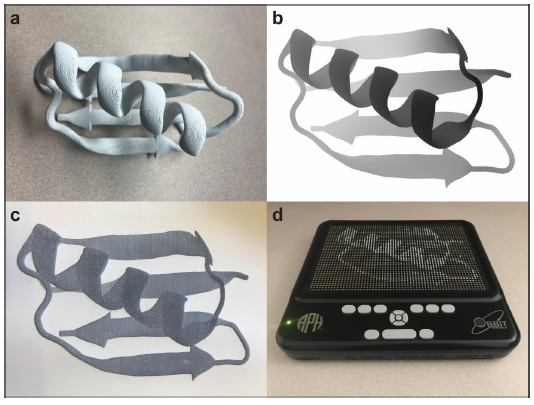
\includegraphics[width=1\linewidth]{fig1.png}
    \caption{Approaches for visualization of protein structures. (a) 3-dimensional printed model. (b) computer rendering with depth-based shading by TactViz. (c) Variable-height tactile graphic produced by TactViz, printed using Picture In A Flash machine. (d) Variable-height tactile visualization using VMD with TactViz on the Graphiti electronic refreshable tactile graphics display.}
    
\end{figure}

Through the development of TactViz, we have enabled an undergraduate student who is blind to carry out publication-quality research on protein structure and structure-function relationships alongside her sighted peers, within the setting of an academic laboratory. The student’s own experience and perspective captures the effectiveness and impact of our tactile visualization strategy:

\begin{quote}
    “By using TactViz in conjunction with the Graphiti, tactile graphics, and 3-dimensional printed models, I have found that the process of research and data analysis is possible with minimal sighted assistance. Particularly advantagious is the text-based command line of the Linux opperating system and VMD text console, which allow for easy use of TactViz with a screen reader and Braille display. While sighted researchers might visualize a protein on a computer screen, I can now perform visualization using tactile approaches. Previously, as a student who is blind, if I was curious about how a particular protein structure looked, I would likely need to ask a sighted teacher or transcriber to describe the protein or help me find a way to make a tactile representation. With TactViz, I can download any protein from the Protein Data Bank, load it into VMD, and use either a tactile graphics printer or tactile graphics display to independently visualize the protein. Independence is critical, particularly for young scientists who are blind who are looking for ways to participate in STEM fields. Most important is the impact our tactile visualization method can have for other students who are blind or visually impaired who are studying the biological sciences, whether at the elementary or advanced level.”
\end{quote}

\section*{SUMMARY}

We have developed TactViz, a VMD plugin to support tactile visualization of proteins, providing a mechanism to produce variable-height tactile graphics of protein structures and improve interactive visualization of protein structures on electronic refreshable tactile graphics display devices. This tool is freely available for download and use and is designed to be accessible to both non-experts and individuals who are blind or visually impaired. Because the plugin can theoretically be used to create tactile graphics of any protein structure in the Protein Data Bank, it provides unprecedented access to tactile training materials relevant to the fields of biology, biochemistry, and biophysics. Furthermore, TactViz has enabled our undergraduate student who is blind to carry out research on protein structure-function relationships alongside her sighted peers. We hope that the tool can serve to reduce barriers to education and research presented by biomolecular visualization for other students, attracting more individuals who are blind or visually impaired to STEM fields and empowering future scientists who do not depend on the sense of sight.

\section*{ACKNOWLEDGEMENTS}

This work was supported by National Science Foundation grant MCB-2027096, funded in part by the Delaware Established Program to Stimulate Competitive Research (EPSCoR). This work used the Extreme Science and Engineering Discovery Environment (XSEDE), which is supported by National Science Foundation grant ACI-1548562, through an Education Allocation TG-SEE200003 on Comet at the San Diego Supercomputer Center. Student support was provided by the Chemical Sciences Leadership Initiative (CSLI) Research Experience for Undergraduates program, funded by National Science Foundation grant CHE-1560325, as well as the XSEDE Expert Mentoring Producing Opportunities for Work, Education, and Research (EMPOWER) program, funded by National Science Foundation grant ACI-1548562. The authors thank Cynthia Yurkovich and Soumita Basu for essential guidance on assistive technology and the production of tactile graphics and Thomas Lum for assistance with 3D printing of protein structures. The authors also thank Orbit Research and the American Printing House for the Blind for loan of a Graphiti prototype. The development of the Graphiti prototype was funded in part by the American Printing House for the Blind and the William M. Wood Foundation.

\end{large}
\clearpage
\section*{REFERENCES}\par 

\leftskip 0.25in
\parindent -0.25in 
Barth, J. L. (1982). \textit{The Tactile Graphics Guidebook}. American Printing House for the Blind, Louisville, KY.

Berman, H. M., Westbrook, J., Feng, Z., Gilliland, G., Bhat, T. N., Weissig, H., \& Shindyalov, I. N. (2000). The Protein Data Bank (www.rcsb.org). \textit{Nucleic Acids Research}. \url{https://doi.org/10.1093/nar/28.1.235}

Buxbaum, E. (2007). \textit{Fundamentals of Protein Structure and Function}. Springer, Boston, MA. \url{https://doi.org/10.1007/978-0-387-68480-2}

Chothia, C. (1984). Principles that Determine the Structure of Proteins. \textit{Annual Review of Biochemistry}. \url{https://doi.org/10.1146/annurev.biochem.53.1.537}

Dobson, C. M. (2019). Biophysical Techniques in Structural Biology. \textit{Annual Review of Biochemistry}. \url{https://doi.org/10.1146/annurev-biochem-013118-111947}

Edman, P. (1992). \textit{Tactile Graphics}. American Foundation for the Blind, New York, NY. \url{https://doi.org/10.1177/026461969201000318}

Goebel, R. (2014). A sketch of a theory of visualization. \textit{Proceedings of the 5th International Conference on Information Visualization Theory and Applications}. \url{https://doi.org/10.5220/0004852702180221}

Goh, B. C., Hadden, J. A., Bernardi, R. C., Singharoy, A., McGreevy, R., Rudack, T., Cassidy, C. K., \& Schulten, K. (2016). Computational Methodologies for Real-Space Structural Refinement of Large Macromolecular Complexes. \textit{Annual Review of Biophysics}. \url{https://doi.org/10.1146/annurev-biophys-062215-011113}

Hashimoto, T., \& Watanabe, T. (2016). \textit{Expansion Characteristic of Tactile Symbols on Swell Paper}. International Conference on Computers Helping People with Special Needs. \url{https://doi.org/10.1007/978-3-319-41267-2\_10}

Humphrey, W., Dalke, A., \& Schulten, K. (1996). VMD: Visual molecular dynamics. \textit{Journal of Molecular Graphics}. \url{https://doi.org/10.1016/0263-7855(96)00018-5}

Rowell, J., \& Ungar, S. (2003). The world of touch: An international survey of tactile maps. Part 1: Production. \textit{British Journal of Visual Impairment}. \url{https://doi.org/10.1177/026461960302100303}

Schmidt, H. L. F., Sperling, L. J., Gao, Y. G., Wylie, B. J., Boettcher, J. M., Wilson, S. R., \& Rienstra, C. M. (2007). Crystal polymorphism of protein GB1 examined by solid-state NMR spectroscopy and X-ray diffraction. \textit{Journal of Physical Chemistry B.} \url{https://doi.org/10.1021/jp075531p}

Thompson, L., \& Chronicle, E. (2006). Beyond visual conventions: Rethinking the design of tactile diagrams. \textit{British Journal of Visual Impairment}. \url{https://doi.org/10.1177/0264619606063400}

\clearpage
\noindent
\begin{large}
\leftskip 0in
\parindent 0in 

\section*{APPENDIX}
This graphic of the protein GB1, rendered by VMD with TactViz, displays an alpha-helix in the foreground and four beta-sheets in the background. Alpha-helices and beta-sheets are major secondary structure elements in proteins. The shape of a protein, defined by its secondary structure and fold, plays an important role in the protein’s function in nature.

\begin{figure}[h]
    \centering
    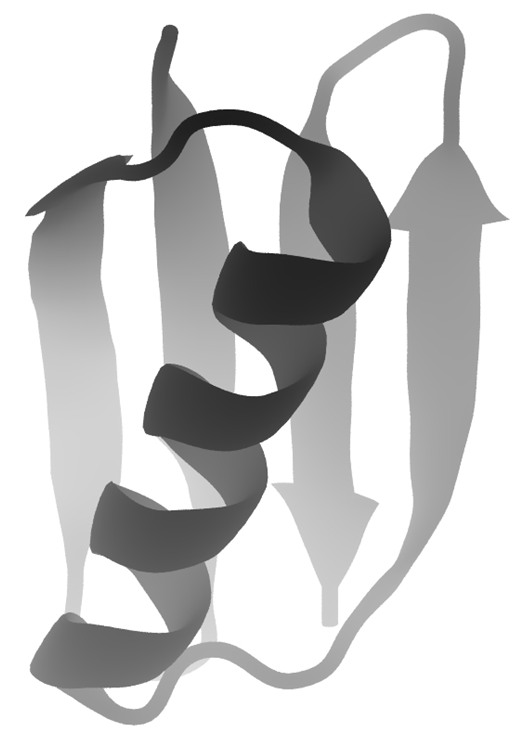
\includegraphics[width=1\linewidth]{fig2.png}
\end{figure}
\end{large}

\end{document}
